\documentclass[aspectratio=169]{beamer}
\input{../flat-blue-theme.inc}
\input{../footnotes.inc}

\usepackage[utf8]{inputenc}
\usepackage[OT1]{fontenc}
\usepackage[ngerman]{babel}
\usepackage{tikz}

\usepackage[outline]{contour}
\contourlength{1.25pt}

\newcommand{\sarrow}{\small$\rightarrow$}
\newcommand{\tipp}[2][Tipp]{\vspace{0.2cm}\textbf{#1:}\\#2}

\setbeamercovered{invisible}
\beamertemplatenavigationsymbolsempty
\setbeamertemplate{title page}[default][right]
\defbeamertemplate*{title page}{customized}[1][]
{
	\raggedleft
	\hspace*{0.5\paperwidth}
	\begin{beamercolorbox}[wd=0.4\paperwidth,ht=4.25ex,dp=2ex]{palette primary}
		\centering\usebeamerfont{title}\inserttitle
	\end{beamercolorbox}
	\restoregeometry
	
	\vspace{1cm}
	\insertauthor\par
	\vspace{1cm}
	\insertdate\par
}

\author{Hauke Stieler\\\href{mailto:4stieler@informatik.uni-hamburg.de}{4stieler@inf}}
\title{Wandern, Trekking \& Co.}
\date{\today}

\begin{document}
	{
		\setbeamertemplate{headline}{}
		\setbeamertemplate{footline}{}
		\setbeamertemplate{background}{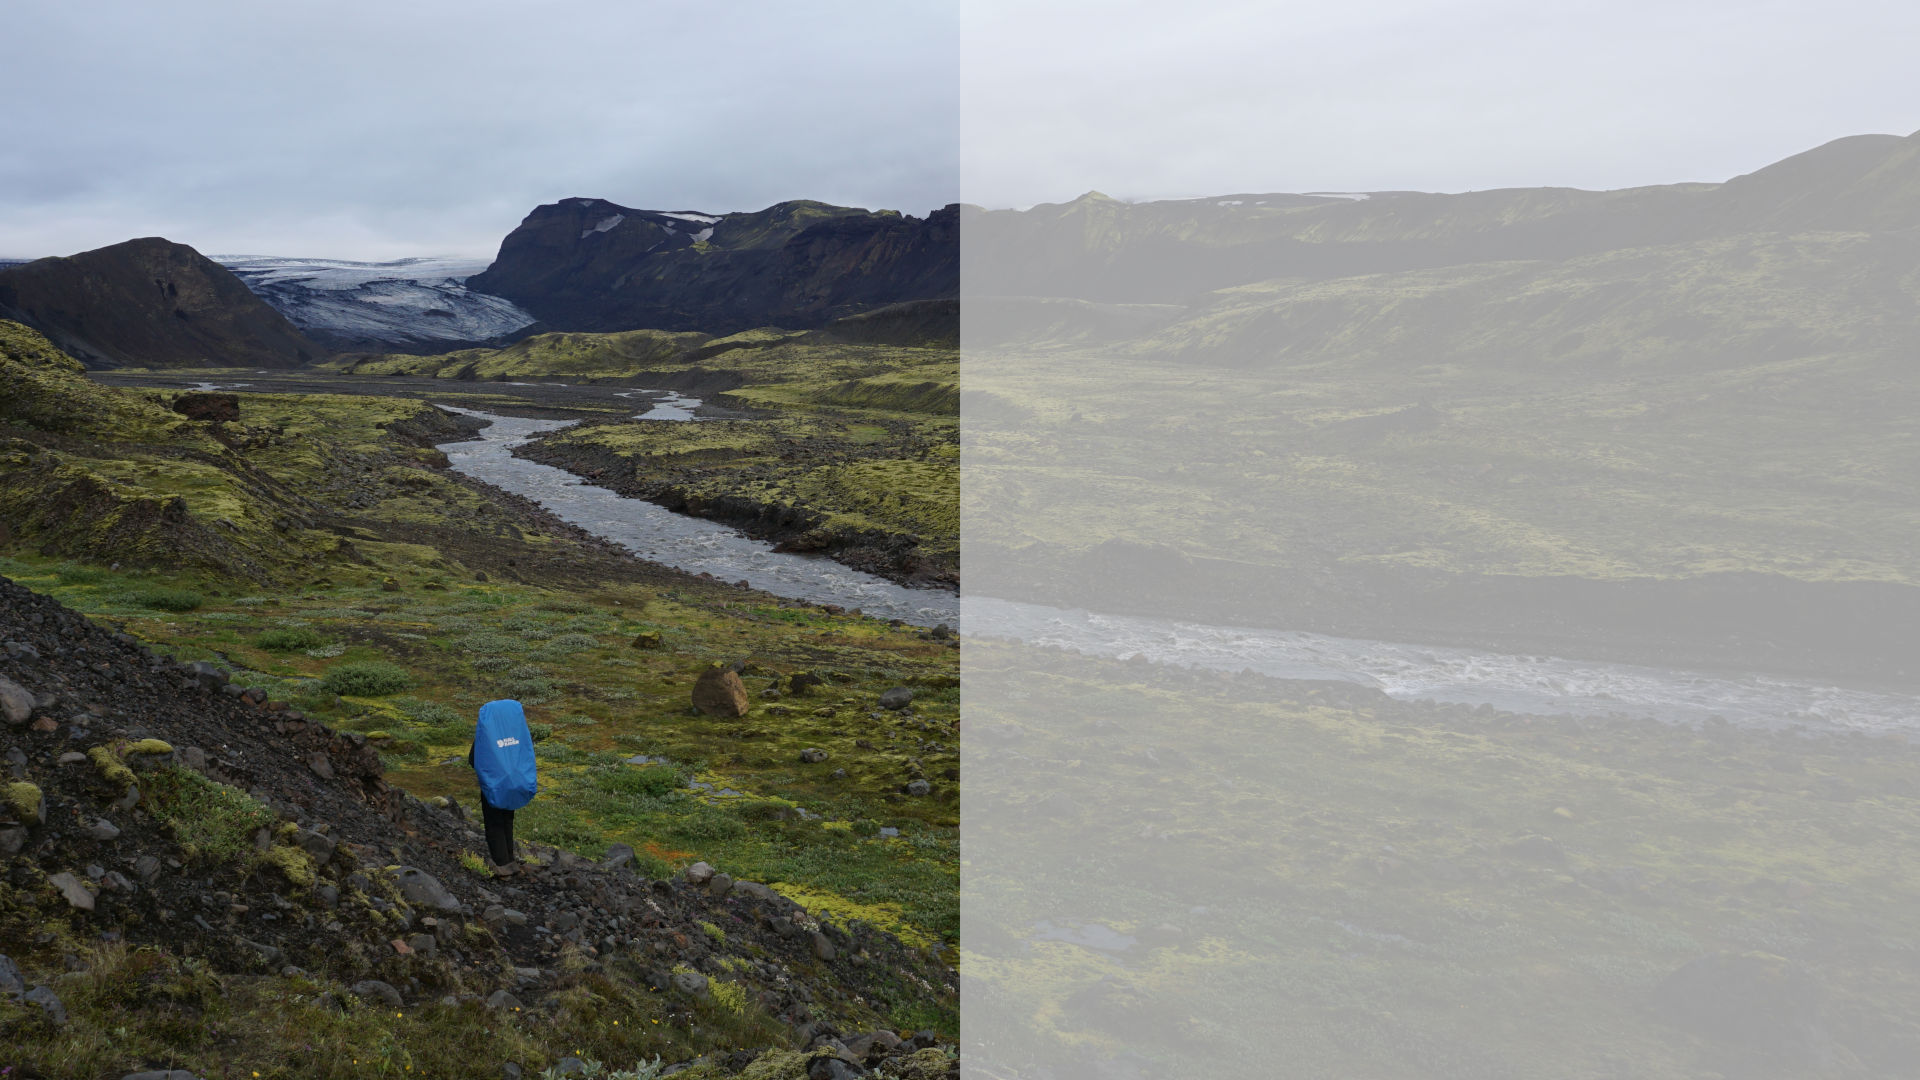
\includegraphics[width=1.01\paperwidth,trim=1 0 0 36]{images/hiking-1}}
		\maketitle
		\addtocounter{page}{-1}
	}
	
	\begin{frame}[t]{Inhalt}
	\tableofcontents[hidesubsections]
	\end{frame}
	
	\section{Grundlagen}
		
		\begin{frame}[t]{Inhalt}
			\tableofcontents[currentsection,hideothersubsections]
		\end{frame}
	
		\subsection{Wandern, Trekking, Bushcrafting ... -- Wo ist der Unterschied?}
		
			\begin{frame}{}
				\begin{itemize}
					\item \textbf{Wandern:} Anspruchsvoller Gang durch die Natur.\pause
					\item \textbf{Trekking:} Mehrtägiges Wandern in (meist) entlegeneren und gebirgigen Gebieten.\pause
					\item \textbf{Bushcrafting:} Nur mit grundlegendem Equipment in einer natürlichen Umgebung zurecht kommen.\pause
					\item \textbf{Thru-Hiking:} End-to-end Wanderung eines langen Wanderweges.\pause
					\item \textbf{Ultraleicht Wandern:} Mit wenig und/oder sehr sehr leichtem Gepäck wandern.
				\end{itemize}
			\end{frame}
		
		\subsection{Wander- \& Tekking-Mythen}
			
			\begin{frame}{}
				\begin{enumerate}
					\item Wandern ist nur was für Outdoor-Freaks / alte Menschen.\pause
					\item Niemals alleine Wandern gehen!\pause
					\item Wandern ist auch nur ein Spatziergang.\pause
					\item Wandern ist total romantisch / entspannend.\pause
					\item Meine wasserdichte GoreTex-Jacke hält mich trocken.\pause
					\item Ohne Profi-Equipment braucht man gar nicht erst anfangen.\pause
					\item Auf längeren Touren muss man Nahrungsergänzungsmittel zu sich nehmen.\pause
					\item Papierkarten? Ich hab doch meine Wander-App.\pause
					\item Wölfe, Bären und Berglöwen wollen mich essen.\pause
					\item Mit einem Erste-Hilfe-Set bin ich sicher.
				\end{enumerate}
			\end{frame}
			
	\section{Equipment \& Navigation}
		
		\begin{frame}[t]{Inhalt}
			\tableofcontents[currentsection,hideothersubsections]
		\end{frame}
		
		\subsection{Equipment}
		
			\begin{frame}{Rucksäcke}
				\begin{itemize}
					\item Maße: Liter (Volumen), Rückenlänge (Passform), Eigengewicht
					\begin{itemize}
						\item Angabe "45+10 L" \textrightarrow\ 45 L Rucksack + 10 L Variabler Anteil
					\end{itemize}\pause
					\item Hüftgurt: Gewichtsverlagerung Schulter \textrightarrow\ Hüfte\pause
					\item Unterschiedliches Design für Frauen \& Männer\pause
					\item Nicht wasserdicht \textrightarrow\ Wasserdichte Regenhülle\pause
					\item Diverse Features: Netz am Rücken, Reißverschlüsse, Außentaschen, Trinksystem, ...
				\end{itemize}
			\end{frame}
			
			\begin{frame}{Rucksäcke: Arten (1/2)}
				\begin{columns}[c]
					\begin{column}{0.64\textwidth}
						\begin{itemize}
							\item \textbf{Tagesrucksäcke}
							\begin{itemize}
								\item Für 0-2 Übernachtungen
								\item Volumen: 5-25 L
								\item Kein oder kleiner Hüftgurt
								\item 30 - 150 €
							\end{itemize}
						\end{itemize}
					\end{column}
					\begin{column}{0.34\textwidth}
						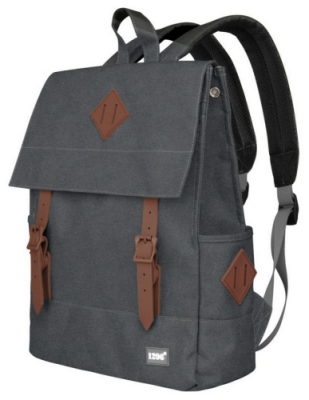
\includegraphics[height=2.25cm]{images/backpack-small.png}
					\end{column}
				\end{columns}
				\vspace{0.4cm}
				\pause
				\begin{columns}[c]
					\begin{column}{0.64\textwidth}
						\begin{itemize}
							\item \textbf{Tourenrucksack}
							\begin{itemize}
								\item Für 1-7 Übernachtungen
								\item Volumen: 25-50 L
								\item Hüftgurt, ggf. Trägersystem
								\item 100 - 300 €
							\end{itemize}
						\end{itemize}
					\end{column}
					\begin{column}{0.34\textwidth}
						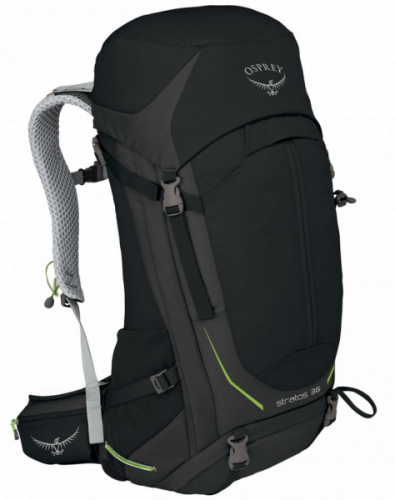
\includegraphics[height=2.5cm]{images/backpack-medium.png}
					\end{column}
				\end{columns}
			\end{frame}
				
			\begin{frame}{Rucksäcke: Arten (2/2)}
				\begin{columns}[T]
					\begin{column}{0.64\textwidth}
						\begin{itemize}
							\item<1-> \textbf{Trekkingrucksack}
							\begin{itemize}
								\item Für 5+ Übernachtungen
								\item Volumen: 45-100 L
								\item Hüftgurt, Trägersystem, ggf. hohes Eigengewicht
								\item 150 - 400 €
							\end{itemize}
							\item<2-> \textbf{Weitere:} Kletterrucksack, Trail-Runner-Rucksack, Skirucksack, ...
						\end{itemize}
					\end{column}
					\begin{column}{0.34\textwidth}
						\onslide<1->{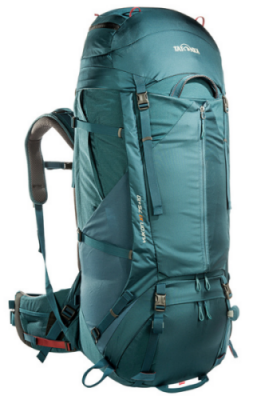
\includegraphics[height=3cm]{images/backpack-big.png}}
					\end{column}
				\end{columns}
			\end{frame}
			
			\begin{frame}{Rucksäcke: Welcher ist der richtige?}
				\begin{itemize}
					\item Was für eine Tour?
					\item Wie viel Equipment?
					\item Wie ist meine Anatomie? \textrightarrow\ Rückenlänge, Hüftbreite, ...
					\item Sind besondere Funktionen nötig/gewünscht?
					\item Tragekomfort \textrightarrow\ Im Laden anprobieren!
				\end{itemize}
			\end{frame}
			
			\begin{frame}{Unterkunft: Zelte \& Tarp}
				\begin{columns}[c]
					\begin{column}{0.69\textwidth}
						\textbf{Zelt:}
						\begin{itemize}
							\item Dach, Wand, Boden + Gestände
							\item Tunnel- / Kuppelzelt
							\item Größe abhängig von Personenanzahl
							\item Sonstige: Autodachzelt, Familienzelt, Strandmuschel, ...\pause
							\item[$+$] Regen, Wind \& Sichtschutz
							\item[$-$] Schwer: 1,5 - 2,5 kg (1-Personen Zelt)
							\item[$-$] Teuer: 200 - 350 €
						\end{itemize}
					\end{column}
					\begin{column}{0.29\textwidth}
						\onslide<1->{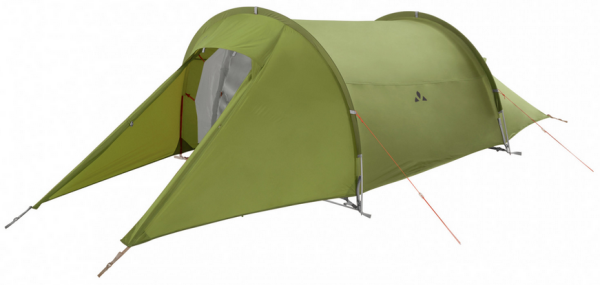
\includegraphics[width=3cm]{images/tent.png}}
					\end{column}
				\end{columns}
			\end{frame}
		
			\begin{frame}{Unterkunft: Zelte \& Tarp}
				\begin{columns}[c]
					\begin{column}{0.69\textwidth}
						\textbf{Tarp:}
						\begin{itemize}
							\item Zelt ohne Gestänge und Boden
							\item Ggf.: Gestände, Seile, Mückennetz, etc.
							\item Dreieckig, Rechteckig, Fünfeckig, ...\pause
							\item[$+$] Leicht(er): $<$ 1 kg (manche sogar $<$ 200 g)
							\item[$+$] Billig(er): ab 6,50 € (bis 300 €)
							\item[$-$] Nicht immer geeignet
						\end{itemize}
					\end{column}
					\begin{column}{0.29\textwidth}
						\onslide<1->{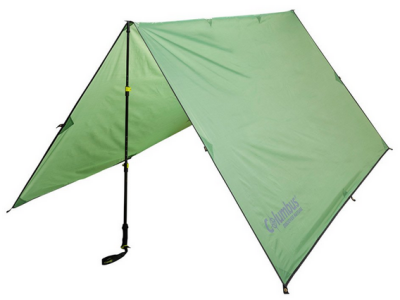
\includegraphics[width=2.5cm]{images/tarp.png}}
					\end{column}
				\end{columns}
				\tipp{Baumarktplane für 6,50 € mit Ösen bei Bauhaus.}
				\end{frame}
				
			\begin{frame}{Unterkunft: Schlafsack}
				\begin{itemize}
					\item Füllmaterial: Kunstfaser vs. Daune
					\item Temperaturbereiche (ISO EN 23537:2016):
					\begin{itemize}
						\item Oberer Grenzbereich: Ab hier schwitzt man.
						\item Komfortbereich: Norm-Frau friert gerade so nicht.
						\item Grenzbereich / Limit: Norm-Mann friert gerade so nicht.
						\item Extrembereich: Norm-Frau überlebt gerade so für 6 Stunden.
					\end{itemize}
				\end{itemize}
				\tipp[Schlafsack Tipp 1]{Am Anfang mit Kunstfaser probieren.}\\\pause
				\tipp[Schlafsack Tipp 2]{Inletts wärmen zusätzlich und verhindern, dass man den eigenen Schlafsack voll schwitzt.}
			\end{frame}
			
			\begin{frame}{Unterkunft: Schlafsack}
				\textbf{Kunstfaser:}
				\begin{itemize}
					\item[$+$] Günstig(er): 100 - 400 € (Herbst- \& Winterschlafsäcke)
					\item[$+$] Können mit Feuchtigkeit umgehen
					\item[$+$] Leichter zu waschen
					\item[$-$] Schwer und Voluminös
				\end{itemize}\pause
				\textbf{Daune:}
				\begin{itemize}
					\item[$+$] Leichter und kleiner
					\item[$-$] Teuer: 300 - 800 € (Herbst- \& Winterschlafsäcke)
					\item[$-$] Daunen verklumpen bei Feuchtigkeit
					\item[$-$] Tricky zu waschen
				\end{itemize}
			\end{frame}
			
			% TODO Temperaturbereiche erklären
			
%			\begin{frame}{Unterkunft: Schlafsack -- Welchen nehmen?}
%				Passender Schlafsack abhängig von ...
%				\begin{itemize}
%					\item[...] erwarteter Temperatur
%					\item[...] erwarteter Feuchtigkeit
%					\item[...] persönlichem Geschmack
%					\item[...] Allergien, etc.
%					\item[...] Toleranz gegenüber Gewicht \& Packmaß
%				\end{itemize}\pause
%				\tipp[Schlafsack Tipp 1]{Am Anfang mit Kunstfaser probieren.}\\\pause
%				\tipp[Schlafsack Tipp 2]{Inletts wärmen zusätzlich und verhindern, dass man den eigenen Schlafsack voll schwitzt.}
%			\end{frame}
			
			\begin{frame}{Unterkunft: Isomatte}
				\begin{itemize}
					\item Mit/ohne Füllmaterial, zusätzliche Isolierung, (selbst) aufblasbar
					\item Wärmeisolierung: R-Wert (gute Isolierung ab $R \geq 3$)
					\item Nicht aufblasbare: 15 - 50€
					\item Aufblasbare: 50 - 300 €
				\end{itemize}\pause
				\tipp[Hinweis]{Ab ca. 5cm Dicke werden Isomatten bequem.}
			\end{frame}
			
%			\begin{frame}{Outdoor-Küche: Geschirr}
%				\begin{itemize}
%					\item Töpfe, Becher, Teller, Flaschen
%					\item Messer, Göffel\footnote{Gabel + Löffel in einem}
%					\item Wasserfilter
%					\item Übliche Materialien: Gummi, Plastik, Alu, Edelstahl, Titan-Legierung
%				\end{itemize}
%			\end{frame}
			
			\begin{frame}{Outdoor-Küche: Kocher (1/2)}
				\begin{columns}[c]
					\begin{column}{0.69\textwidth}
						\textbf{Gaskocher:}
						\begin{itemize}
							\item Kartusche mit Isobutan, Propan, etc.
							\item Aufsatz für Kartusche
							\item[\sarrow] Allrounder, billig, einfache Benutzung, Kartuschen ggf. nicht immer verfügbar
						\end{itemize}
					\end{column}
					\begin{column}{0.29\textwidth}
						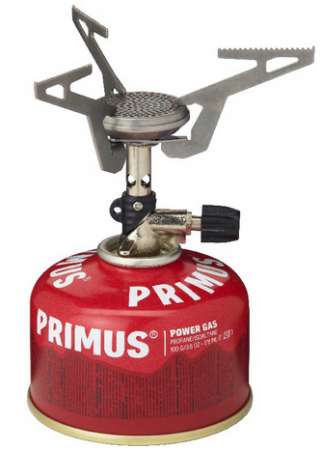
\includegraphics[width=2.5cm]{images/kocher-gas.png}
					\end{column}
				\end{columns}
			\end{frame}
				
			\begin{frame}{Outdoor-Küche: Kocher (2/4)}
				\begin{columns}[c]
					\begin{column}{0.69\textwidth}
						\textbf{Spirituskocher:}
						\begin{itemize}
							\item Becher für Spiritus
							\item Gestell für Topf
							\item[\sarrow] Simpler Aufbau, keine Kartusche, Spiritus überall verfügbar, Vorsicht bei Benutzung
						\end{itemize}
					\end{column}
					\begin{column}{0.29\textwidth}
						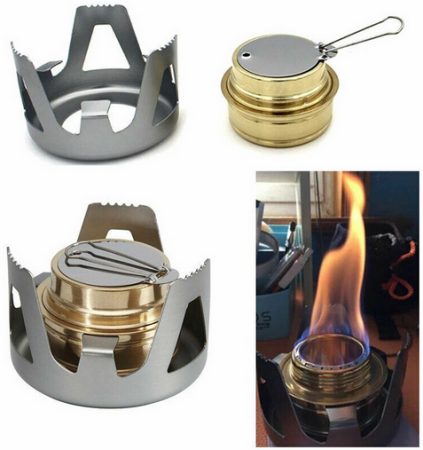
\includegraphics[width=3cm]{images/kocher-spiritus.png}
					\end{column}
				\end{columns}
			\end{frame}
		
			\begin{frame}{Outdoor-Küche: Kocher (3/4)}
				\begin{columns}[c]
					\begin{column}{0.62\textwidth}
						\textbf{Benzinkocher / Mehrstoffkocher:}
						\begin{itemize}
							\item Drucktank für Benzin (alternativ: Petroleum, Diesel, Kerosin)
							\item Vorheiz-Filz
							\item Brennkopf mit Halterung für Topf
							\item[\sarrow] Schwierige Handhabung, hohe Heizleistung, Brennstoff überall verfügbar
						\end{itemize}
					\end{column}
					\begin{column}{0.36\textwidth}
						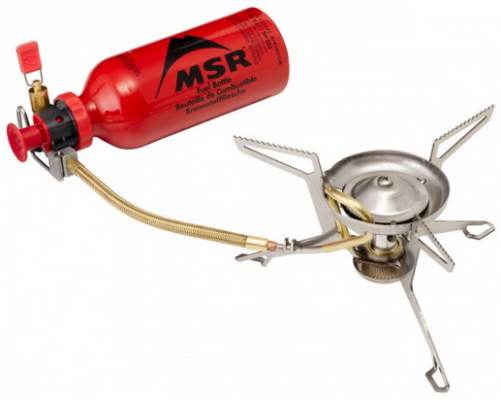
\includegraphics[width=3.85cm]{images/kocher-benzin.png}
					\end{column}
				\end{columns}
			\end{frame}
		
			\begin{frame}{Outdoor-Küche: Kocher (4/4)}
				\begin{columns}[c]
					\begin{column}{0.69\textwidth}
						\textbf{Hobokocher:}
						\begin{itemize}
							\item Kleiner Holzofen
							\item Ineinander gesteckte Bleche
							\item[\sarrow] Kleines Packmaß, Brennstoff Verfügbarkeit prüfen, ggf. illegal (z.B. in NSGs) 
						\end{itemize}
					\end{column}
					\begin{column}{0.29\textwidth}
						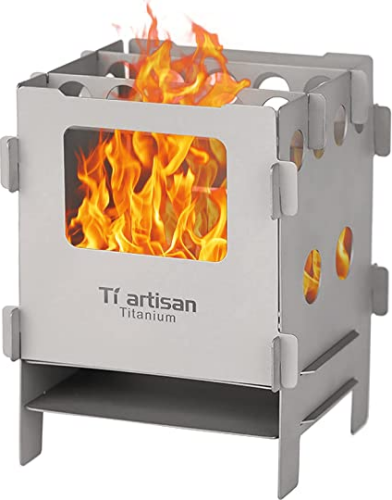
\includegraphics[width=2.35cm]{images/kocher-hobo.png}
					\end{column}
				\end{columns}
			\end{frame}
			
			\begin{frame}{Outdoor-Essen: Frühstück}
				\begin{itemize}
					\item Müsli / Porridge
					\item Rührei aus Eipulver und Wasser
					\item Tee, Instant-Kaffeepulver
					\item[\sarrow] Gerne warm, viele Kohlenhydrate \& Proteine, mäßig viel Fett, wenig/kein Zucker
				\end{itemize}\pause
				\tipp{Aufstehen, eine Stunde wandern und erst dann Frühstücken}\\\pause
			\end{frame}
			
			\begin{frame}{Outdoor-Essen: Snacks}
				\begin{itemize}
					\item Müsli- oder Sportriegel (\textrightarrow\ möglichst wenig Zucker!)
					\item Nüsse
					\item Trockenfrüchte
					\item Fruchtleder, Beef Jerky
					\item Kekse, Cracker, Knäckebrot
					\item Dunkle Schokolade
				\end{itemize}
			\end{frame}
			
			\begin{frame}{Outdoor-Essen: Hauptmahlzeit}
				\begin{itemize}
					\item Warme \& leckere Mahlzeit
					\item Idealerweise: Getrocknetes Essen, heißes Wasser drauf, ziehen lassen, fertig\pause
					\item Fertigprodukte:
					\begin{itemize}
						\item Sea To Summit, Trek'n Eat, ...
						\item Teuer + viel Müll
					\end{itemize}\pause
					\item Selbst mischen:
					\begin{itemize}
						\item Nudeln, Linsen, Reis, Cousous, Bulgur, Quinoa, getr. Tofu, Haferflocken
						\item Getrocknetes Gemüse, Röstzwiebeln, Samen, Kerne
						\item Eine Tüte Fertiggericht-, Suppen- oder Saucenpulver
						\item Kleines Fläschchen Öl separat mitnehmen
					\end{itemize}
					\item Nachtisch hebt die Stimmung (und liefert Kalorien)
				\end{itemize}
			\end{frame}
			
			\begin{frame}{Outdoor-Essen: Hinweise}
				\begin{itemize}
					\item Kalorienverbrauch x1,5 bis x2 ($>$ 2500-3000 / Tag)
					\begin{itemize}
						\item Fertig-Gerichte: 500 - 700 kcal
						\item Eigene Mischung: ca. 300-350 kcal / 100g
						\item Gewichtsabnahme bei längeren Wanderungen wahrscheinlich
					\end{itemize}
					\item Gerade bei längeren Touren: Es muss schmecken!
				\end{itemize}
			\end{frame}
			
			\begin{frame}{Hygiene}
				\textbf{Must have:}
				\begin{itemize}
					\item Zahnputzsachen, Waschlappen, Handtuch (Mikrofaser)
					\item Outdoor-Seife (einigermaßen biologisch abbaubar)
					\item Toilettenpapier
					\item Erste-Hilfe-Set, Desinfektionsmittel
				\end{itemize}\pause
				\textbf{Optional:}
				\begin{itemize}
					\item Deo
					\item Schlafsack Inlett
				\end{itemize}\pause
				\textbf{Überbewertet (IMHO):}
				\begin{itemize}
					\item Parfum, Schmuck, Schminke o.O
					\item Schampoo, Duschgel
				\end{itemize}
			\end{frame}
			
			\begin{frame}{Werkzeuge}
				\begin{itemize}
					\item Kompass
					\item Taschenmesser, Multitool, Axt
					\item Taschenlampe, Stirnlampe
					\item Feuerzeug (besser: Feuerstahl)
				\end{itemize}
			\end{frame}
			
			\begin{frame}{Kleidung: Materialien}
				\begin{itemize}
					\item Baumwolle (\textrightarrow\ \textit{cotton kills}), Viskose, Lyocell
					\item Wolle (Schaf, Merino, Alpaka, etc.)
					\item Polyesther, Polypropylen
					\item Nylon
					\item Membrane (GoreTex, H2NO, Drilite, etc.)
				\end{itemize}
			\end{frame}
			
			\begin{frame}{Kleidung}
				\begin{itemize}
					\item Unterwäsche: Normale oder Funktionsunterwäsche
					\item Mütze, Hut, Multifunktions / Tunneltuch
					\item Top, T-Shirt, Langarmshirt, Sport-Shirts
					\item Jacke: Normal, Soft- / Hardshell, Regenjacke
					\begin{itemize}
						\item Poncho
					\end{itemize}
					\item Hose: Normal, Soft- / Hardshell, Regenhose
					\item Wandershuhe / -stiefel
					\item Wandersocken
				\end{itemize}
			\end{frame}
				
			\begin{frame}{Kleidung}
				\textbf{Hinweise zu Regenjacken:}
				\begin{itemize}
					\item Sind i.d.R. auch winddicht
					\item Bleiben nicht wasserdicht!
				\end{itemize}
				\pause
				\vspace{0.2cm}
				\textbf{Hinweise zu Blasen:}
				\begin{itemize}
					\item Verursacht durch Reibung
					\item Begünstigt durch Wärme \& Feuchtigkeit
					\item Zwei-Socken-Strategie: Normale Socken und darüber Wandersocken
				\end{itemize}
			\end{frame}
			
			\begin{frame}{Kleidung}
				\textbf{Must have:}
				\begin{itemize}
					\item Bequeme Kleidung
					\item An Witterung, Temperatur, Umgebung, Dauer, Belastung angepasst
					\item Immer trockene Wechselkleidung!
					\item Passendes Schuhwerk (\textrightarrow\ gute Wanderschuhe)
					\item Socken-Strategie, die keine Blasen verursacht
				\end{itemize}\pause
				\textbf{Optional:}
				\begin{itemize}
					\item Funktionskleidung
				\end{itemize}\pause
				\textbf{Überbewertet (IMHO):}
				\begin{itemize}
					\item Gewisse Marken (z.B. Icebreaker, Fjällräven, Arc'teryx)
				\end{itemize}
			\end{frame}
			
			\begin{frame}{Wanderstöcke}
				\begin{columns}[c]
					\begin{column}{0.69\textwidth}
						\begin{itemize}
							\item<1->[$+$] Mehr Stabilität \& Trittsicherheit
							\item<1->[$+$] Gewichtsverlagerung
							\item<1->[$+$] Weniger anstrengend
							\item<1->[$+$] Geringere Kniebelastung
							\item<1->[$+$] Hilfreich beim Furten
							\item<1->[$+$] Gestände beim Tarp
							\item<2->[$-$] Hände nicht mehr frei
							\item<2->[$-$] Falsche Sicherheit
							\item<2->[$-$] Schäden an Weg und Natur
						\end{itemize}
					\end{column}
					\begin{column}{0.29\textwidth}
						\onslide<1->{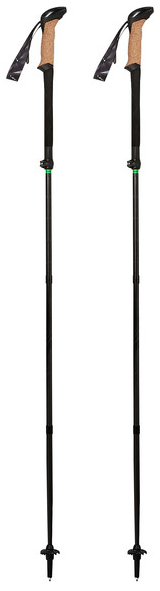
\includegraphics[width=1.25cm]{images/hiking-sticks.png}}
					\end{column}
				\end{columns}
			\end{frame}
		
		\subsection{Karten}
			
			\begin{frame}{Arten}
				\begin{minipage}{0.59\textwidth}
					\textbf{Relevante Rubriken:}
					\begin{itemize}
						\item<1-> Stadtpläne, Straßenkarten
						\item<1-> Fahrradkarten
						\item<1-> Gewässerkarten
						\item<2-> Luftbildkarten
						\item<3-> Thematische Karten
						\item<4-> Wanderkarten
						\item<4-> Topografische Karten
					\end{itemize}
				\end{minipage}
				\begin{minipage}{0.39\textwidth}
					\onslide<1->{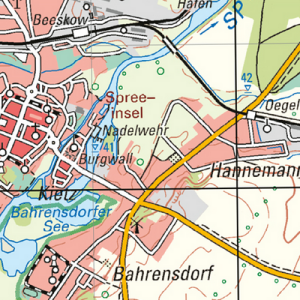
\includegraphics[height=2cm]{images/map-example-street.png}}
					\onslide<2->{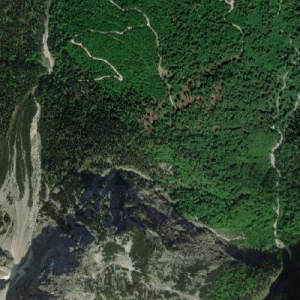
\includegraphics[height=2cm]{images/map-example-aerial.png}}\vspace{0.1cm}\\\noindent
					\onslide<3->{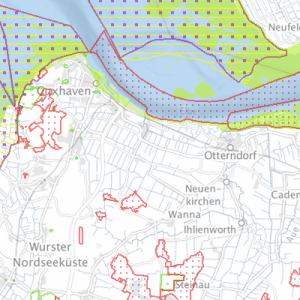
\includegraphics[height=2cm]{images/map-example-thematic.png}}
					\onslide<4->{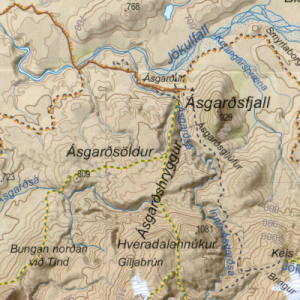
\includegraphics[height=2cm]{images/map-example-hiking.png}}
				\end{minipage}
			\end{frame}
			
			\begin{frame}{Bestandteile}
				\begin{minipage}{0.59\textwidth}
					\begin{itemize}
						\item<1-> Legende
						\item<2-> Maßstab
						\item<3-> Koordinaten
						\item<4-> Ggf. Nordpfeil
					\end{itemize}
				\end{minipage}
				\begin{minipage}{0.39\textwidth}
					\onslide<1->{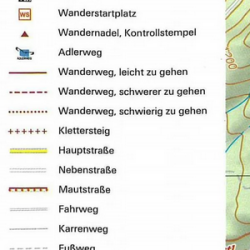
\includegraphics[height=2cm]{images/map-legend.png}}
					\onslide<2->{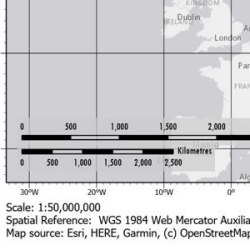
\includegraphics[height=2cm]{images/map-scale.png}}\vspace{0.1cm}\\\noindent
					\onslide<3->{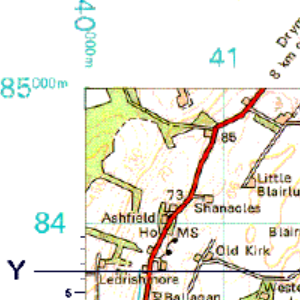
\includegraphics[height=2cm]{images/map-coordinates.png}}
					\onslide<4->{
\includegraphics[height=2cm]{images/map-north-arrow.png}}
				\end{minipage}
			\end{frame}
			
			\begin{frame}{Topografische Karten lesen (1/2)}
				\begin{center}
					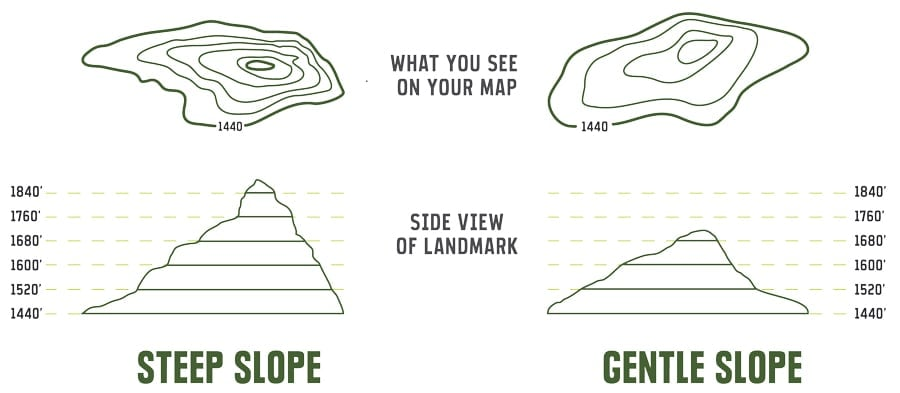
\includegraphics[width=0.8\textwidth]{images/map-topo-rei.jpg}
				\end{center}
				{\hfill\tiny Bildquelle: \href{https://www.rei.com/learn/expert-advice/topo-maps-how-to-use.html}{rei.com}}
			\end{frame}
			
			\begin{frame}{Topografische Karten lesen (2/2)}
				\begin{center}
					\begin{tikzpicture}
						[
							font=\scriptsize
						]
						\node[anchor=south west,inner sep=0] (image) at (0,0) {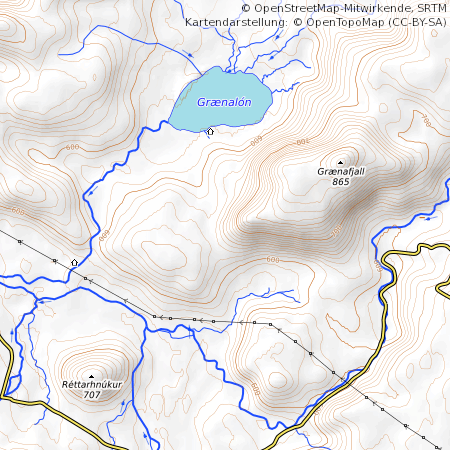
\includegraphics[height=0.75\textheight]{images/map-topo-base.png}};
						
						\begin{scope}[x={(image.south east)},y={(image.north west)}]
%							\draw[help lines,xstep=.1,ystep=.1] (0,0) grid (1,1);
%							\foreach \x in {0,1,...,9} { \node [anchor=north] at (\x/10,0) {\tiny 0.\x}; }
%							\foreach \y in {0,1,...,9} { \node [anchor=east] at (0,\y/10) {\tiny 0.\y}; }
							
							\only<1>{
								\node[red] (gipfel) at (0.5, 0.05) {\contour{white}{Gipfel}};
								\draw[thick,red,->] (gipfel) -- (0.21,0.16);
								\draw[thick,red,->] (gipfel) -- (0.37,0.43);
							}
							
							\only<2>{
								\node[red] (valley) at (0.3, 0.05) {\contour{white}{Tal}};
								\draw[thick,red,->] (valley) -- (0.22,0.46);
								\draw[thick,red,->] (valley) -- (0.5,0.27);
								\node[red] (saddle) at (0.75, 0.05) {\contour{white}{Sattel}};
								\draw[thick,red,->] (saddle) -- (0.48,0.45);
								\draw[thick,red,->] (saddle) -- (0.7,0.31);
							}
							
							\only<3>{
								\node[red] (flat) at (0.5, 0.05) {\contour{white}{Flache Ebene}};
								\draw[thick,red,->] (flat) -- (0.19,0.31);
								\draw[thick,red,->] (flat) -- (0.37,0.65);
							}
							
							\only<4>{
								\node[red] (gentle) at (0.5, 0.05) {\contour{white}{Seichter Anstieg}};
								\draw[thick,red,->] (gentle) -- (0.175,0.48);
								\draw[thick,red,->] (gentle) -- (0.95,0.27);
							}
							
							\only<5>{
								\node[red] (gentle) at (0.38, 0.05) {\contour{white}{Steiler Anstieg}};
								\draw[thick,red,->] (gentle) -- (0.42,0.32);
								\node[red] (cliff) at (0.72, 0.05) {\contour{white}{Klippe}};
								\draw[thick,red,->] (cliff) -- (0.64,0.44);
							}
							
							\only<6>{
								\node[red] (view) at (0.5, 0.05) {\contour{white}{Geile Aussicht}};
								\draw[thick,red,->] (view) -- (0.05,0.56);
								\draw[thick,red,->] (view) -- (0.56,0.51);
								\draw[thick,red,->] (view) -- (0.63,0.62);
							}
						\end{scope}
					\end{tikzpicture}
				\end{center}
			\end{frame}
		
		\subsection{Navigation}
			
			\begin{frame}{Equipment}
				\begin{minipage}{0.59\textwidth}
					\begin{itemize}
						\item<1-> Karte \& Kompass
						\begin{itemize}
							\item Kartenausrichtung
							\item Orientierung, Wegfindung
							\item Positionsbestimmung
						\end{itemize}
						\item<2-> Handy, GPS-Gerät
						\item<3-> Sonne, Mond, Sterne
						\item<3-> Uhr
						\begin{itemize}
							\item Orientierung mit Uhrzeit und Sonne
						\end{itemize}
					\end{itemize}
				\end{minipage}
				\begin{minipage}{0.39\textwidth}
					\only<1>{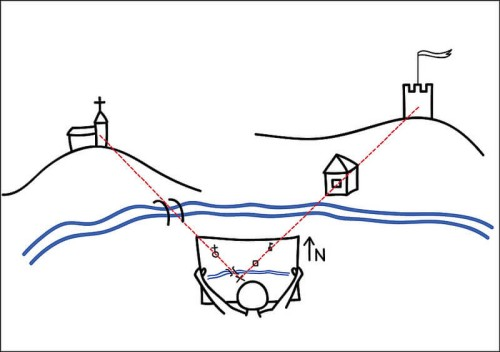
\includegraphics[width=4cm]{images/navigation-map-positioning.jpg}}
					\only<2>{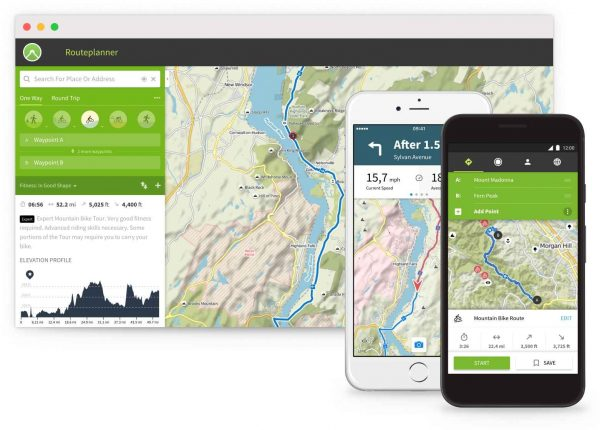
\includegraphics[width=4cm]{images/navigation-app.jpg}}
					\only<3>{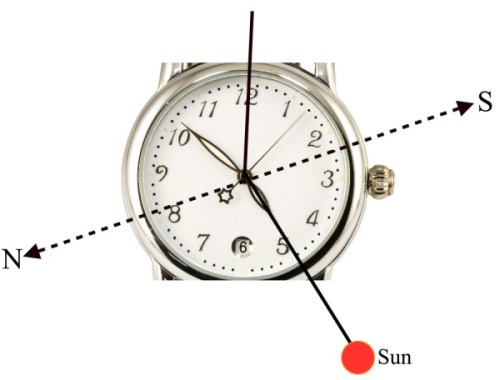
\includegraphics[width=4cm]{images/navigation-clock-sun.jpg}}
				\end{minipage}
			\end{frame}
	
	\section{Tourenplanung}
		
		\begin{frame}[t]{Inhalt}
			\tableofcontents[currentsection,hideothersubsections]
		\end{frame}
		
		\begin{frame}{Informationsquellen}
			\begin{columns}[T]
				\begin{column}{0.55\textwidth}
					\begin{itemize}
						\item<1-> Routenplaner (z.B. \href{https://classic-maps.openrouteservice.org/}{openrouteservice.org})
						\item<2-> Luftbilder (Google Maps, Bing, Esri, amtliche, etc.)
						\item<2-> Wanderführer, Wanderkarten
						\item<3-> Lokale Websites, Tourismusverbände, etc.
						\item<3-> Foren, Reddit, AllTrails, WikiLoc, Komoot, etc.
					\end{itemize}
				\end{column}
				\begin{column}{0.44\textwidth}
					\only<1>{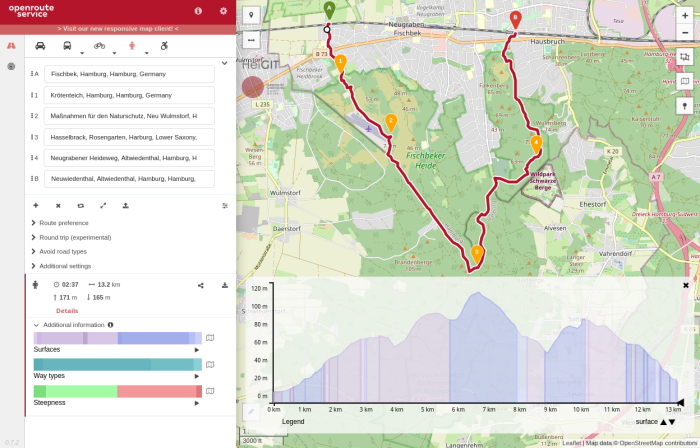
\includegraphics[width=0.95\linewidth]{images/info-source-routing-1.png}}
					\only<2->{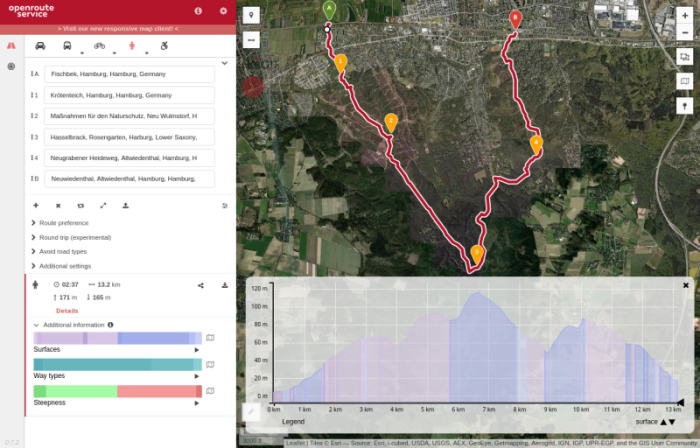
\includegraphics[width=0.95\linewidth]{images/info-source-routing-2.png}}
				\end{column}
			\end{columns}
		\end{frame}
		
		\begin{frame}{Equipment}
			Was sollte \textit{immer} mit?
			\begin{itemize}
				\item Rucksack
				\item Adäquates Schuhwerk
				\item Erste-Hilfe-Set (FAK -- First-Aid-Kit)
				\item Karte (ggf. sonstiges Navigationsequipment)
				\item Handy (ggf. Powerbank oder Solarzelle)
				\item Trinken / Trinkflasche
			\end{itemize}\pause
			Was sollte \textit{meistens} noch mit?
			\begin{itemize}
				\item Regenkleidung
				\item Wechselkleidung
			\end{itemize}
		\end{frame}
		
		\begin{frame}{Planung}
			\begin{itemize}
				\item Geplante Route \& Verlauf überlegen
				\item Schwierigkeit abschätzen, ggf. Route anpassen
				\item Eigene Geschwindigkeit \& Fähigkeiten beachten
				\item Passendes Equipment einplanen
				\item Wichtige Dokumente dabei haben (Tickets, Karten, etc.)
				\item Im Ausland:
				\begin{itemize}
					\item Notrufnummer kennen\footnote{In Deutschland natürlich 112. Bergwacht, Seenotrettung, etc. ggf. abweichende Nummern.}
					\item Visum, Impfungen, Einreisebestimmungen, Bargeld, etc.
				\end{itemize}
				\item Familie, Bekannte, etc. über Tour informieren!
				\item Benötigte Fähigkeiten kennen, auffrischen, lernen
			\end{itemize}
		\end{frame}
	
		\subsection{Tagestouren}
		
			\begin{frame}
				\vspace{1cm}
				\begin{center}
					\textcolor{blue}{\textbf{Tagestouren}}
					\\\,\\
					{\scriptsize 1-2 Tage}
				\end{center}
			\end{frame}
			
			\begin{frame}{Planung}
				Sollte immer geplant werden:
				\begin{itemize}
					\item An- \& Abreise
					\item Genug Essen \& vor allem Trinken einpacken
					\item Reicht die Zeit?
				\end{itemize}
				Je nach Situation prüfen/einplanen:
				\begin{itemize}
					\item Sonnenaufgang / -untergang prüfen
					\item Equipment für ein Notcamp / -biwak
				\end{itemize}
			\end{frame}
			
			\begin{frame}{Equipment}
				Sollte immer dabei sein
				\begin{itemize}
					\item Alles zuvor erwähnte (Rucksack, FAK, Karte, etc.)
				\end{itemize}
				Je nach Situation einpacken:
				\begin{itemize}
					\item Regen- / Wechselkleidung
					\item Equipment für ein Notcamp
				\end{itemize}
			\end{frame}
			
		\subsection{Mehrtägige Touren}
		
			\begin{frame}
				\vspace{1cm}
				\begin{center}
					\textcolor{blue}{\textbf{Mehrtägige Touren}}
					\\\,\\
					{\scriptsize 2-7 Tage}
				\end{center}
			\end{frame}
		
			\begin{frame}{Planung}
				Sollte immer geplant werden:
				\begin{itemize}
					\item An- \& Abreise
					\item Etappen
					\item Unterkünfte (wild campen, Campingplätze, Hütten, etc.)
					\item Verpflegung
					\item Verfügbarkeit von Wasser prüfen
					\item Kurz vorher: Wetterbericht + ggf. Kleidung anpassen
				\end{itemize}
				Je nach Situation prüfen / einplanen:
				\begin{itemize}
					\item Alternativrouten
				\end{itemize}
			\end{frame}
			
			\begin{frame}{Equipment}
				Sollte immer dabei sein
				\begin{itemize}
					\item Alles zuvor erwähnte (Rucksack, FAK, Karte, etc.)
					\item Unterkunft (Tarp, Zelt, Hütten-Buchung, etc.) + Schlafsachen
					\item Kocher
					\item Genug Wechselkleidung
					\item Passende Hygiene-Artikel
				\end{itemize}
				Je nach Situation einpacken:
				\begin{itemize}
					\item Utensilien zum Feuer machen
				\end{itemize}
			\end{frame}
		
		\subsection{Mehrwöchige Touren}
		
			\begin{frame}
				\vspace{1cm}
				\begin{center}
					\textcolor{blue}{\textbf{Mehrwöchige Touren}}
					\\\,\\
					{\scriptsize 7-28 Tage}
				\end{center}
			\end{frame}
		
			\begin{frame}{Planung (1/2)}
				Sollte immer geplant werden:
				\begin{itemize}
					\item Alles zuvor erwähnte (An-/Abreise, Etappen, Unterkünfte, etc.)
					\item Gewicht vom Equipment beachten
					\item Kontaktmöglichkeiten vor Ort (Internet, Mobilfunk, Münz-Telefon, Post, ...)
					\item Reise Freunden \& Familie bekannt geben
					\item Körperliche Fitness sicherstellen\footnote{ab ins Gym, bro}
					\item Mit Equipment vertraut sein
				\end{itemize}
			\end{frame}
				
			\begin{frame}{Planung (2/2)}
				Je nach Situation prüfen/einplanen:
				\begin{itemize}
					\item Wohnung Urlaubssicher machen (Haustiere, Lebensmittel, Heizung, etc.)
					\item Post Nachsendeauftrag, Verträge pausieren, autom. E-Mail Antwort
					\item Erste-Hilfe-Kurs besuchen
					\item Versicherungen prüfen
					\begin{itemize}
						\item Krankenversicherungsschutz im Ausland
						\item Reiserücktrittsversucherung
						\item Kosten für Rettung/Bergung beachten
					\end{itemize}
				\end{itemize}
			\end{frame}
			
			\begin{frame}{Equipment}
				Sollte immer dabei sein
				\begin{itemize}
					\item Alles zuvor erwähnte
					\item Noch mehr Essen, Brennstoff, Kleidung
				\end{itemize}
				Je nach Situation:
				\begin{itemize}
					\item Verpflegung / Equipment an strategischen Punkten deponieren
				\end{itemize}
			\end{frame}
	
	\section{Richtiges Verhalten}
		
		\begin{frame}[t]{Inhalt}
			\tableofcontents[currentsection,hideothersubsections]
		\end{frame}
		
		\subsection{Verhaltensweisen: Do's \& Don'ts}
			
			\begin{frame}{Do's}
				\begin{itemize}
					\item Sich gut vorbereiten
					\item Adäquates Equipment eingepackt haben
					\item Nicht alleine schwierige Touren machen
					\item Backup-Pläne haben
					\item Reisepläne anderen mitteilen
					\item Gesetze befolgen (z.B. bzgl. Naturschutzgebiete)
					\item Toilettenpapier mitnehmen, verbrennen oder notfalls vergraben
				\end{itemize}
			\end{frame}
			
			\begin{frame}{Don'ts}
				\begin{itemize}
					\item Müll vor Ort liegen lassen
					\item Feuer machen, wenn es nicht klug / erlaubt ist
					\item Musik an haben
					\item Zu anspruchsvolle Touren machen
					\item Sich drauf verlassen, dass man ja immer gerettet werden kann
					\item Je nach Situation: Jagen, Pflanzen beschädigen / essen
					\item Wasserquellen verschmutzen
				\end{itemize}
				\pause
				\vspace{0.2cm}
				\textcolor{blue}{\textrightarrow}\ Leave no trace!
			\end{frame}
			
			\begin{frame}{Do's \& Don'ts untereinander}
				\begin{itemize}
					\item Rücksicht auf andere nehmen
					\begin{itemize}
						\item Nett Grüßen
						\item Wer hoch geht hat Vorrang
						\item Abstand zwischen Camps / Zelten
					\end{itemize}
					\item Anderen nicht auf den Senkel gehen
					\item Anbieten Essen zu teilen, aber nicht danach fragen
					\item Nicht flirten!
				\end{itemize}
			\end{frame}
			
		\subsection{Sicherheit}
			
			\begin{frame}{}
				\begin{itemize}
					\item Gute Planung!
					\item Adäquates Equipment
					\begin{itemize}
						\item Schuhwerk, Kleidung, Sicherungen, etc.
						\item An Wetter, Temperatur und Gegebenheiten angepasst
						\item Erste-Hilfe-Set
						\item Karte, Handy / GPS-Gerät
					\end{itemize}
					\item Limits kennen
					\item Nötige Skills können (Navigation, Furten, Erste-Hilfe, Feuermachen, ...)\pause
					\item Gesunder Menschenverstand
				\end{itemize}
			\end{frame}
	
	\section{Rechtliches, Tipps \& Tricks}
		
		\begin{frame}[t]{Inhalt}
			\tableofcontents[currentsection,hideothersubsections]
		\end{frame}
	
		\subsection{Rechtliche Lage}
			
			\begin{frame}{In Deutschland}
				Allgemein:
				\begin{itemize}
					\item Wald:
					\begin{itemize}
						\item Darf zur Erholung betreten werden
						\item Offene Feuer verboten
						\item Nicht geschützte Pflanzen dürfen verzehrt werden
					\end{itemize}
					\item Wild Zelten / Campen
					\begin{itemize}
						\item Im Wald: Verboten
						\item Auf offener Landschaft: Je nach Bundesland verboten
						\item Biwakieren: Teilw. geduldet
						\item[\textrightarrow] Trekkingplätze
					\end{itemize}
				\end{itemize}
			\end{frame}
			
			\begin{frame}{In Deutschland}
				Schutzgebiete:
				\begin{itemize}
					\item Wege nicht verlassen
					\item Übernachten verboten
					\item Feuermachen verboten
					\item Pflanzen nicht abpflücken oder beschädigen
				\end{itemize}
				\vspace{0.2cm}
				\textcolor{blue}{\textrightarrow}\ \href{https://geodienste.bfn.de/schutzgebiete}{geodienste.bfn.de/schutzgebiete}\\
				\pause
				\vspace{0.2cm}
				\tipp[Hinweis]{Notbiwaks / -camps sind \textit{immer} erlaubt}
			\end{frame}
			
			\begin{frame}{International}
				\begin{itemize}
					\item Sehr sehr verschieden
					\item Jedermannsrecht\footnote{Engl. \textit{freedom to roam}}:
					\begin{itemize}
						\item Schottland, Schweden, Norwegen, Finnland, Estland
						\item Rest von Europa eher nicht
						\item International eher selten (in Kanada und Neuseeland teilw.)
					\end{itemize}
				\end{itemize}
			\end{frame}
%		
		\subsection{Tipps \& Tricks}
		
			\begin{frame}{}
				\begin{itemize}
					\item Mit wenig \& einfachem Equipment anfangen
					\item Mit kurzen \& leichten Touren anfangen
					\item Poncho $>$ Regenjacke
					\item Wanderschuhe vorher einlaufen
					\item Zwei-Socken-Strategie
				\end{itemize}
			\end{frame}
		
		{
			\setbeamertemplate{headline}{}
			\setbeamertemplate{footline}{}
			\setbeamertemplate{background}{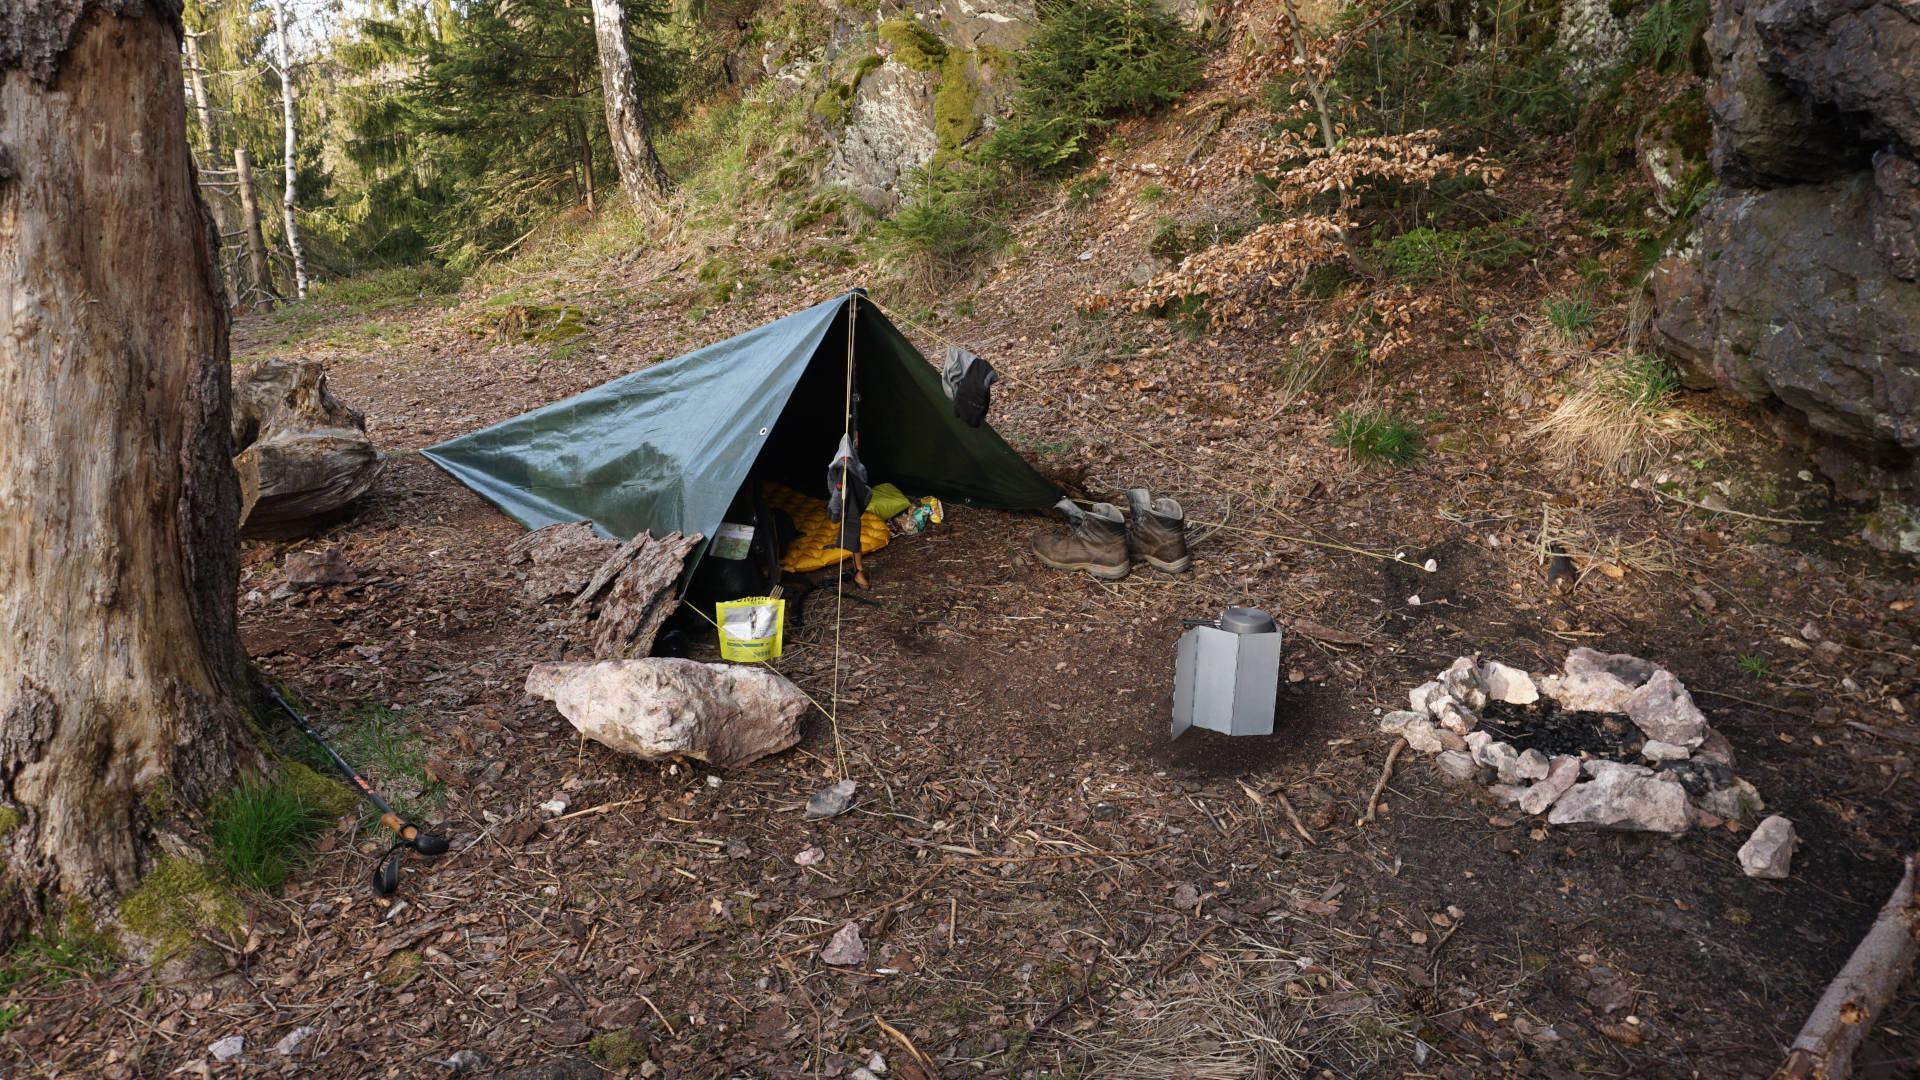
\includegraphics[width=1.01\paperwidth,trim=1 0 0 36]{images/hiking-2}}
			\frame{}
		}
\end{document}